\RequirePackage{mathtools, amssymb, amsmath, amsfonts}
% A0 portrait poster.
\documentclass[25pt, a0paper, portrait, margin=15mm, innermargin=15mm,
               blockverticalspace=12mm, colspace=12mm, subcolspace=8mm]{tikzposter}

\usepackage[utf8]{inputenc}
\usepackage[english]{babel}
\usepackage{bm}
\usepackage{graphicx}
\graphicspath{{../figures/}{./}}
\usepackage{tikz}
\usetikzlibrary{arrows.meta, positioning, calc, decorations.pathreplacing}
\usepackage{enumitem}
\usepackage{multicol}
\setlist[itemize]{leftmargin=*, itemsep=1pt, topsep=1pt, parsep=0pt}
\setlist[enumerate]{leftmargin=*, itemsep=1pt, topsep=1pt, parsep=0pt}

\newcommand{\reals}{\mathbb{R}}
\newcommand{\vv}[1]{\mathbf{#1}}
\newcommand{\DD}{\vv{D}}
\newcommand{\yy}{\vv{y}}
\newcommand{\xx}{\vv{x}}
\newcommand{\xxi}{\boldsymbol{\xi}}
\newcommand{\Bsp}{\mathcal{B}}

\definecolor{navy}{HTML}{152B4A}
\definecolor{ink}{HTML}{1F2A3A}
\definecolor{accent}{HTML}{00008C}
\definecolor{accentsoft}{HTML}{DCE0F0}
\definecolor{cream}{HTML}{FAF6EE}
\definecolor{paper}{HTML}{FFFFFF}
\definecolor{rule}{HTML}{D6D2C7}
\definecolor{muted}{HTML}{6E6A60}

\usetheme{Default}\useblockstyle{Default}\usetitlestyle{Empty}\usebackgroundstyle{Empty}
\colorlet{backgroundcolor}{cream}\colorlet{framecolor}{cream}
\colorlet{titlebgcolor}{cream}\colorlet{titlefgcolor}{navy}
\colorlet{blocktitlebgcolor}{cream}\colorlet{blocktitlefgcolor}{navy}
\colorlet{blockbodybgcolor}{paper}\colorlet{blockbodyfgcolor}{ink}
\colorlet{innerblocktitlebgcolor}{accentsoft}\colorlet{innerblocktitlefgcolor}{navy}

\defineblockstyle{Editorial}{
  titlewidthscale=1, bodywidthscale=1, titleleft,
  titleoffsetx=0pt, titleoffsety=0pt, bodyoffsetx=0pt, bodyoffsetx=0pt,
  bodyverticalshift=2mm, roundedcorners=0, linewidth=0pt,
  titleinnersep=0pt, bodyinnersep=4pt
}{
  \draw[draw=rule, fill=blockbodybgcolor, line width=0.6pt]
       (blockbody.south west) rectangle (blockbody.north east);
}
\useblockstyle{Editorial}

\newcommand{\stepbadge}[1]{%
  \tikz[baseline=(N.base)]{
    \node[circle, fill=accent, text=white, font=\sffamily\bfseries\small,
          inner sep=0pt, minimum size=1.0em] (N) {#1};}%
}
\newcommand{\bt}[2]{{\normalsize\stepbadge{#1}\hspace{0.5em}\sffamily\bfseries\color{navy}\MakeUppercase{#2}}}
\newcommand{\btnonum}[1]{{\normalsize\rule[-0.4em]{0pt}{1.0em}\sffamily\bfseries\color{navy}\MakeUppercase{#1}}}

\settitle{%
  \noindent
  \begin{minipage}[t]{0.96\textwidth}\vspace{0pt}
    {\color{navy}\bfseries\fontsize{50}{58}\selectfont
       Spike Coding Networks as Piecewise Projective Maps:~Closed-Form Stable Periodic Firing Patterns\par}
    \vspace*{5mm}
    {\color{ink}\large
      \begin{minipage}[t]{0.65\textwidth}\raggedright
        \'Abel S\'agodi \;\textbullet\; Ildefonso Ferreira Pica \;\textbullet\; William Podlaski \textbullet\; Champalimaud Foundation
      \end{minipage}%
      \hfill
      \begin{minipage}[t]{0.32\textwidth}\raggedleft
        Dynamics Days Europe 2026, Lisbon\par
      \end{minipage}%
    }
  \end{minipage}\hfill
  % \\[6mm]
  % \noindent\begin{minipage}{\linewidth}
  %   {\sffamily\bfseries\large\color{accent}TL;DR.}\;
  %   {\color{ink}\normalsize
  %     SCN dynamics reduce \emph{exactly} to a piecewise \textbf{projective map}
  %     $\xxi'=(\vv{A}\xxi+\vv{b})/(\vv{c}^\top\xxi+d)$ on the spike-bound hyperplanes.
  %     Composing per-spike matrices along a firing word $\sigma$ yields a \textbf{symbolic return map} $\vv{M}_\sigma$; its leading eigenvector is the periodic orbit.
  %     The \emph{inverse problem}, finding drives $\bm{\alpha}$ that realize a desired $\sigma$, has an analytical solution.}
  % \end{minipage}%
}

\tikzposterlatexaffectionproofoff
\title{~}\author{~}\institute{~}

\begin{document}
\maketitle[width=0.97\textwidth, titletotopverticalspace=5mm,
          titletoblockverticalspace=6mm]

% ============================================================
% ROW 1: Setup + Projective Map (MERGED, full width)
% ============================================================
\begin{columns}
\column{0.5}
\block{\bt{0}{Background}}{
\begin{minipage}[t]{\linewidth}\vspace{0pt}\normalsize
\textbf{Abstract:} Since the discovery that neurons communicate via discrete spikes~\ref{ref:adrian}~\ref{ref:hodgkin} a central goal of neuroscience has been to link ensemble spiking patterns to computations and behavior. Spike coding networks (SCNs)--a class of recurrent spiking neural networks--combine principles of efficient coding and neurobiology to yield dynamical models that produce spiking patterns with which these networks approximate arbitrary nonlinear input-output mappings~\ref{ref:podlaski}. SCNs remain interpretable through the geometric properties~\ref{ref:calaim} of their governing equations. We derive a discrete-time mapping of the continuous-time SCN framework to address two open questions: (1) Which periodic firing patterns are produced by a given SCN? (2) Can we construct a SCN that reliably produces a desired firing pattern?

\textbf{SNN dynamics:} Consider a network of 2 recurrently connected spiking neurons. We denote each neuron's membrane potential by $\vv{V}_i$ and assume that the neuron fires a spike when it reachtes a threshold, $\vv{T}$. The membrane potential dynamics will be described using the leaky integrate-and-fire (LIF) neuron model:

\vspace{5mm}
\begin{center}
$\tau\dot{\vv{V}}_i(t)=-\vv{V}_i(t)+\vv{F}_i\vv{c}(t)+\sum_{j=1}^{K=2}\vv{W}_{ij}\vv{s}_j(t)+\vv{b}_i<\vv{T}_i\longrightarrow \vv{V}_i=\vv{F}_i \xx+\sum_{j=1}^{K=2}\vv{E}_i\vv{D}_j\vv{r}_j<\vv{T}_i$
\end{center}
\end{minipage}\hfill
\vspace{5mm}
\begin{center}
\resizebox{\linewidth}{!}{%
  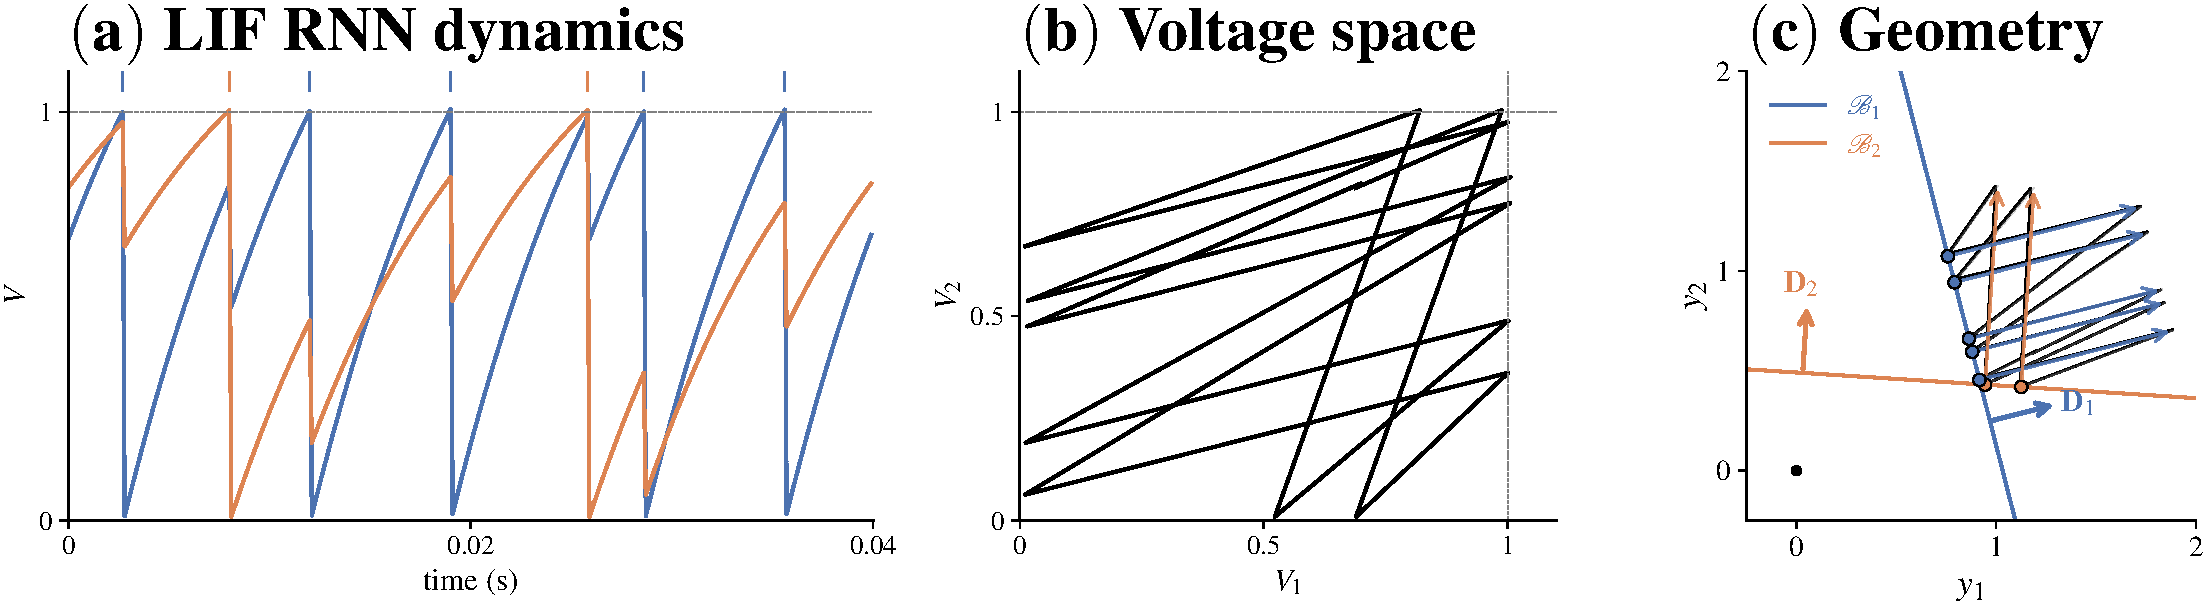
\includegraphics[height=5.5cm]{two_neuron_voltages.pdf}\hspace{2mm}
  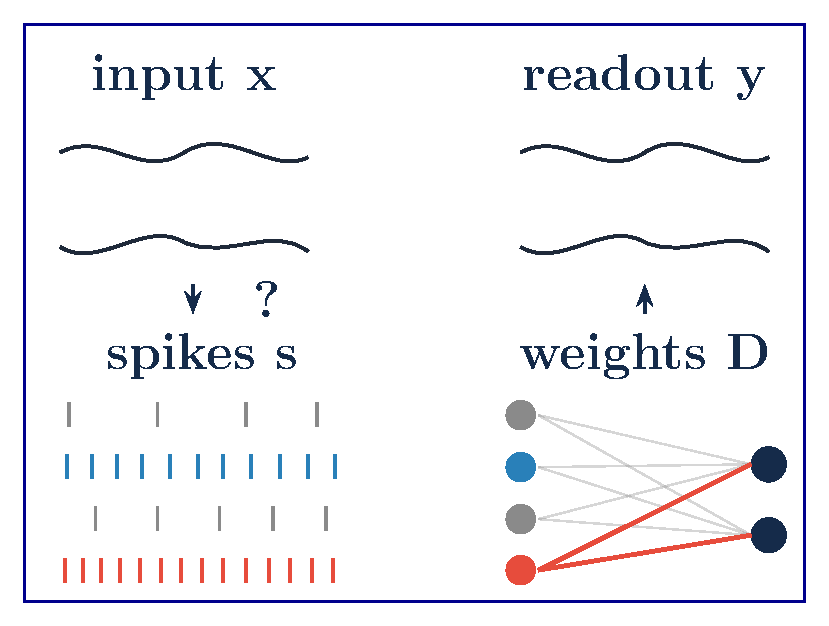
\includegraphics[height=5.5cm]{scn_schematic.pdf}%
}
\end{center}\normalsize
\textbf{Autoencoder SCN:} Now consider a network that generates spike patterns such that an input signal $\xx(t)$ can be approximately recovered using a linear combination of the spikes:~$\yy(t)=\sum_{i=1}^{K}\DD_ir_i(t)$. Setting $F{=}E{=}D^\top$ we can interpret the neuron's voltage as a geometric projection of the readout error:~$\vv{V}_i=\vv{D}_i^\top\left(\xx-\yy\right)$~\ref{ref:boerlin}, \ref{ref:calaim}.
}
\column{0.5}
\block{\bt{1}{Setup \& Inter-bound Geometry}}{\normalsize
\textbf{Definitions:} $K$ neurons encode $\xx\in\reals^N$ via readout $\yy = \vv{D}\vv{r}$:
decay $\dot\yy = -\lambda\yy$; spike $\yy \mapsto \yy + \DD_i$ at $\DD_i^\top\yy = \alpha_i$. With $\vv{U}_i$ the tangent frame of $\Bsp_i$ (its $N{-}1$ columns span the hyperplane):
$\cos\psi_{ji}=\DD_j^\top\DD_i$ (decoder cosine);\;
$\vv{v}_{ji}=\vv{U}_i^\top\DD_j$, $\;\vv{w}_{ji}=\vv{U}_j^\top\DD_i$ (decoders projected into the tangent frames);\;
$\vv{R}_{ji}=\vv{U}_j^\top\vv{U}_i$ (maps tangent frame $i\!\to\!j$).
\begin{center}
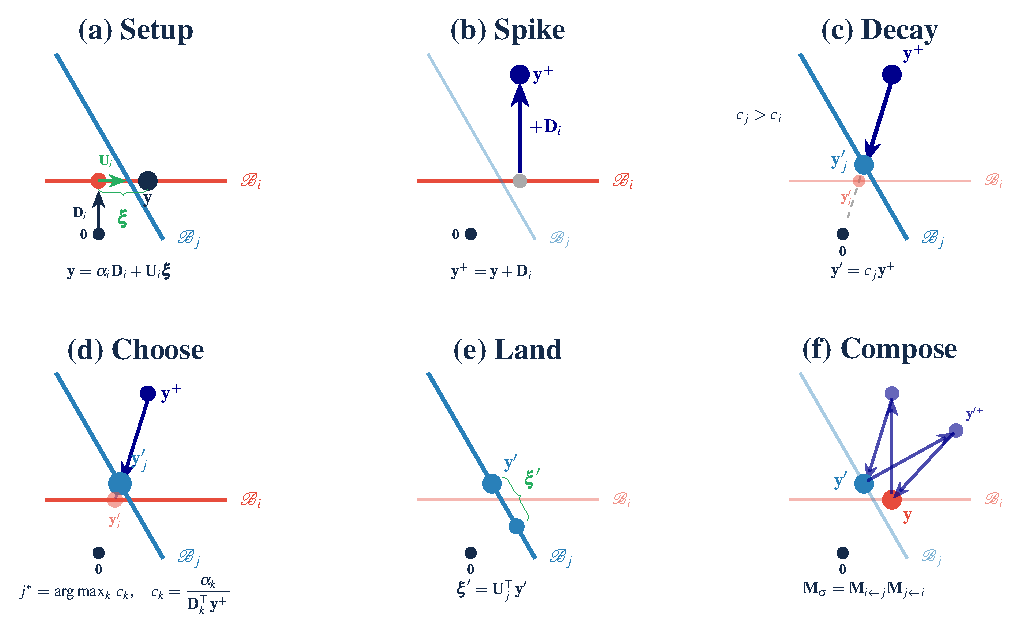
\includegraphics[width=0.861\linewidth]{derivation_tikz.pdf}
\end{center}
}
\end{columns}

% ============================================================
% ROW 2: Two-Neuron Overview & Maps + Orbits as eigenvectors
% ============================================================
\begin{columns}
\column{0.5}
\block{\bt{3}{Analysis of a Two-Neuron system}}{
\begin{minipage}[t]{\linewidth}
\centering
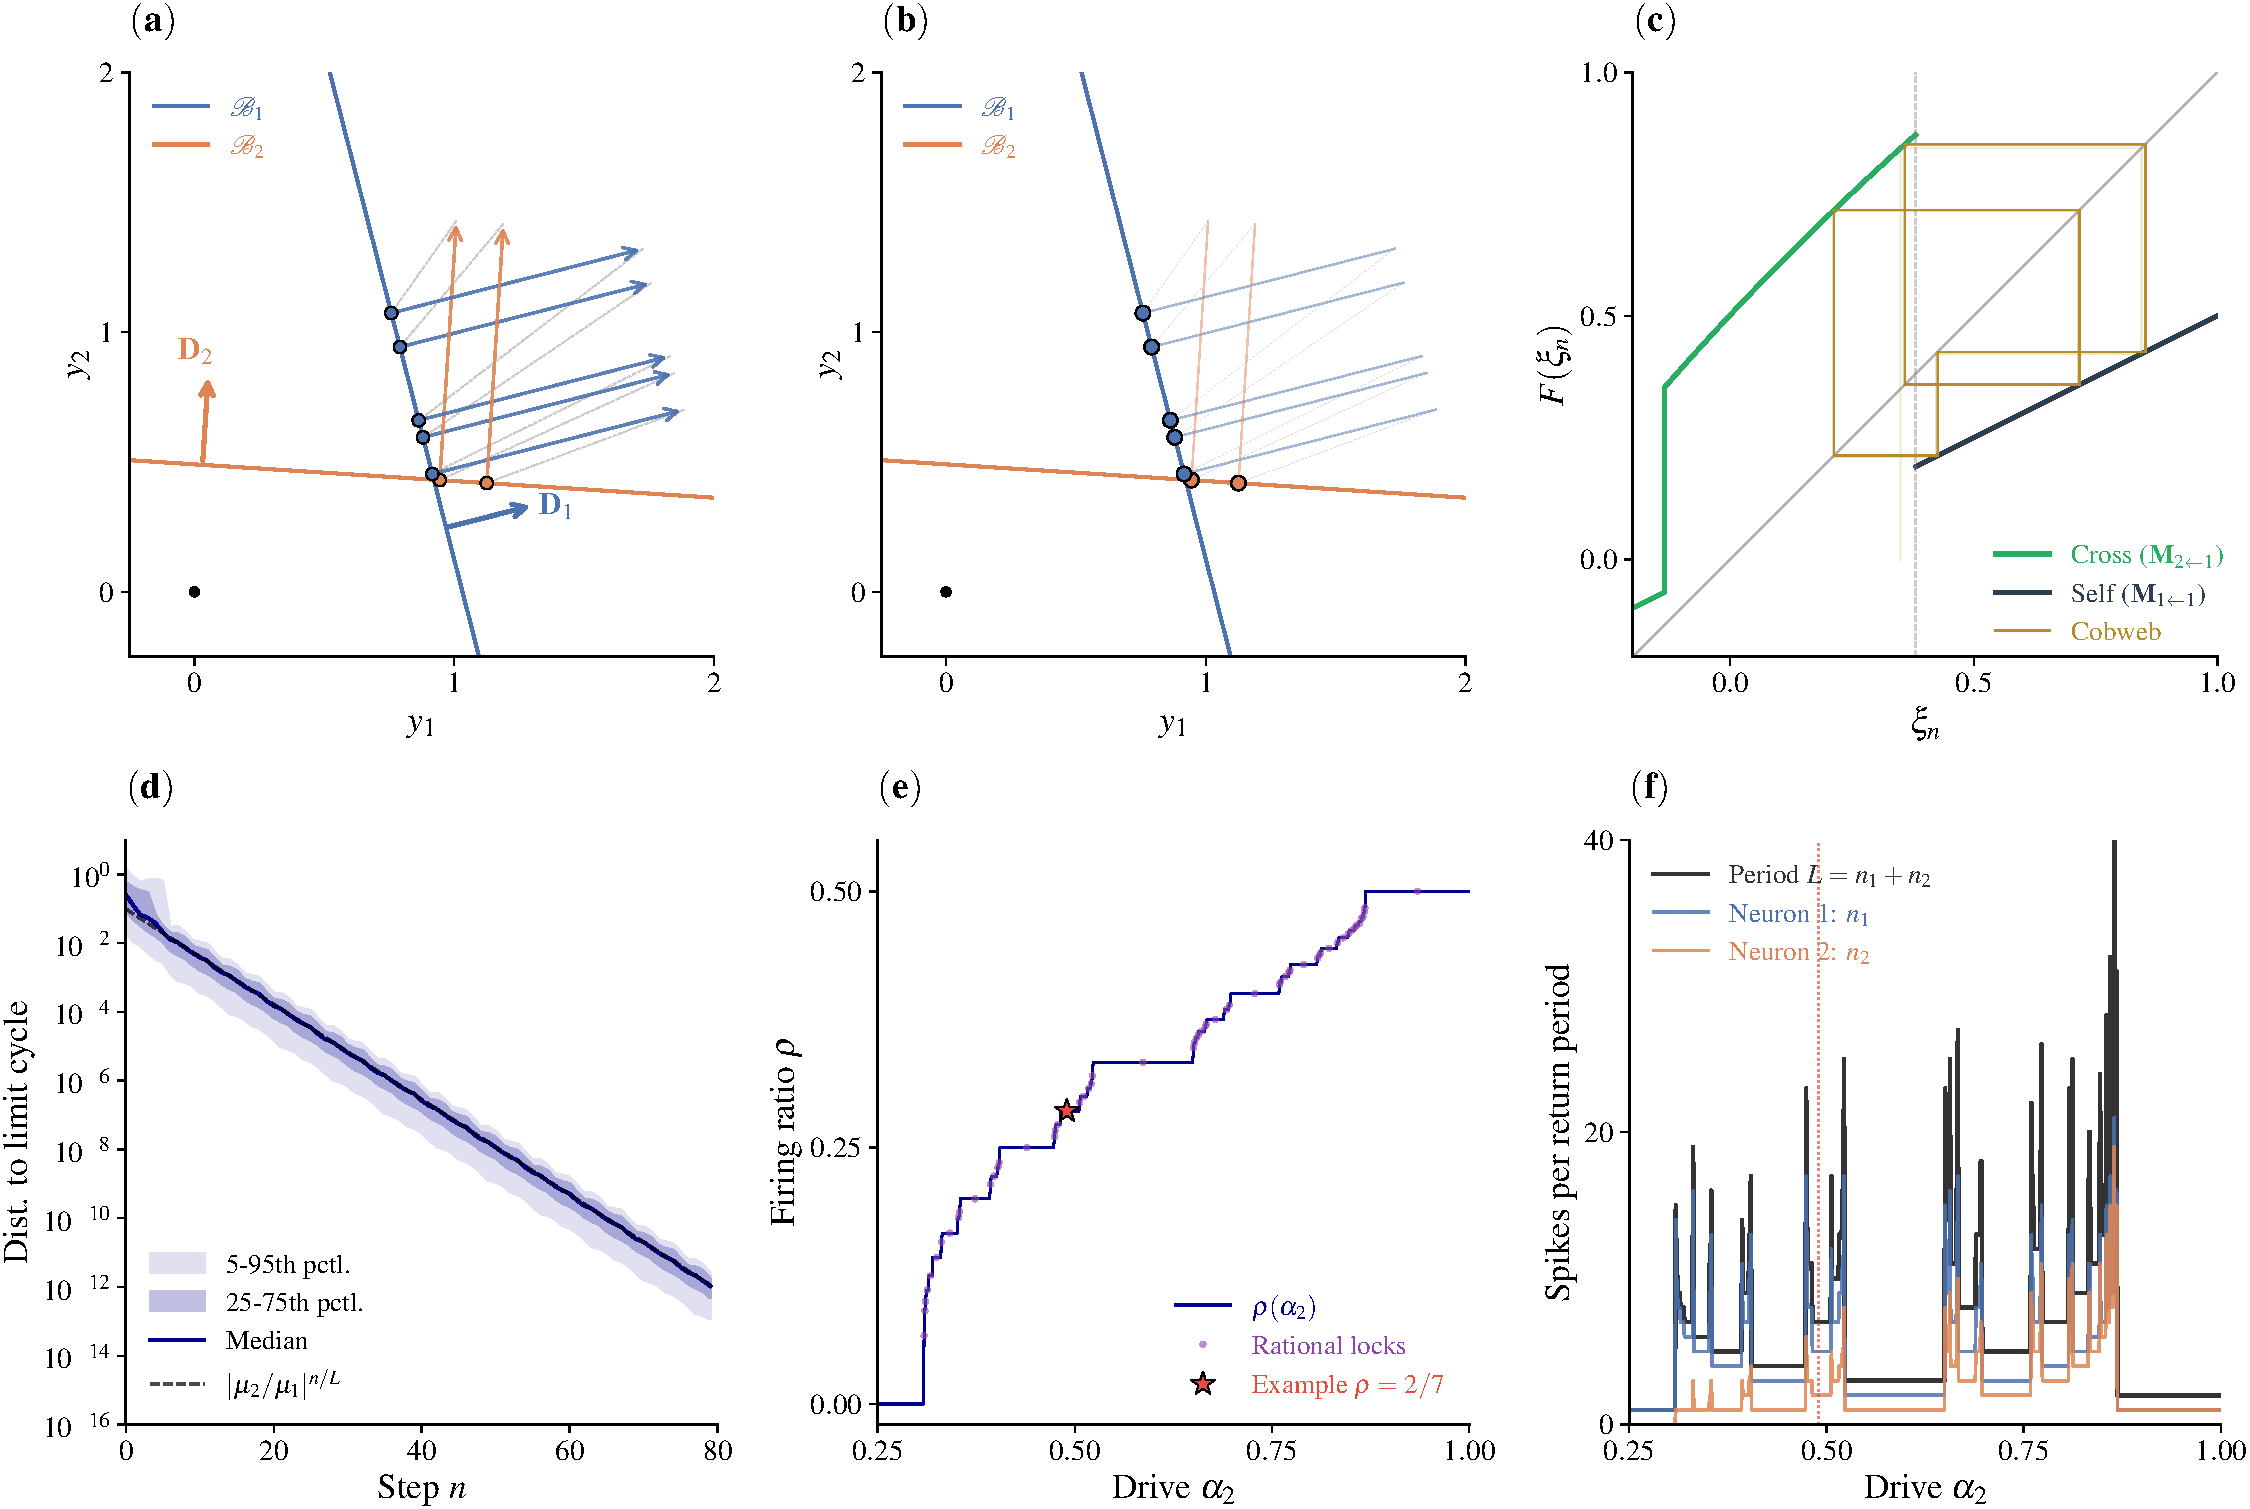
\includegraphics[width=0.96\linewidth]{scn_word_example.pdf}
\end{minipage}
}

\column{0.5}
\block{\bt{2}{Projective map, return map and periodic orbits as eigenvectors}}{
\begin{minipage}[t]{\linewidth}\normalsize
\textbf{Aim:} Derive discrete-time mapping of the continuous-time SCN and analyze SCN periodic behavior.

\textbf{Derivation:} We rewrite the expression of the single-step evolution of the network state (in tangent coordinates) into matrix form using homogeneous coordinates, resulting in a projective map:

\begin{center} %: a point on $\Bsp_i$ is mapped to the next firing bound $\Bsp_j$ via the formula below.
$\displaystyle\xxi_j = \alpha_j\,\frac{(\alpha_i{+}1)\vv{w}_{ji}+\vv{R}_{ji}\,\xxi_i}{(\alpha_i{+}1)\cos\psi_{ji}+\vv{v}_{ji}^\top\xxi_i}$
\quad$\longrightarrow$\quad
$\vv{M}_{j\leftarrow i} = \begin{pmatrix} \alpha_j\vv{R}_{ji} & \alpha_j(\alpha_i{+}1)\vv{w}_{ji} \\ \vv{v}_{ji}^\top & (\alpha_i{+}1)\cos\psi_{ji} \end{pmatrix}$
\end{center}

Each spike bound $\Bsp_i \subset \reals^N$ is an $(N{-}1)$-dim hyperplane. On $\Bsp_i$: $\yy = \alpha_i\DD_i + \vv{U}_i\xxi$, where $\xxi\in\reals^{N-1}$ is the tangent coordinate. The full dynamics is a \emph{piecewise projective map} on the disjoint union $\bigsqcup_i \Bsp_i$.

\textbf{Results:} \emph{1. Symbolic return map:} For a firing word $\sigma=(b_0,\ldots,b_{L-1})$, composing the per-spike matrices $\vv{M}_{b_{k+1}\leftarrow b_k}$ gives the return map $\vv{M}_\sigma = \prod_{k} \vv{M}_{b_{k+1}\leftarrow b_k} \in \reals^{N\times N}$, which propagates the tangent coordinate $\xxi\in\Bsp_{b_0}$ once around the cycle.

\emph{2. Periodic orbit $\leftrightarrow$ eigenvector:} Picture the homogeneous coordinate $\tilde\xxi=(\xxi^{*\top},1)^\top$ as a ray through the origin of $\reals^N$, and $\xxi^*$ as the unique point where this ray pierces the affine slice $\{x_N{=}1\}$. A period-$L$ cycle returns the ray to itself, $\vv{M}_\sigma\tilde\xxi^*=\mu_1\tilde\xxi^*$: $\xxi^*$ is the dehomogenization of the dominant eigenvector. The scale $\mu_1$ does not move the pierce point and cancels.

\emph{3. Stability spectrum:} The return map $F=\mathrm{dh}\circ\vv{M}_\sigma$ on $\Bsp_{b_0}$ has, at its fixed point $\xxi^*$, a Jacobian with $N{-}1$ eigenvalues. Numerator $\mu_k$ along a transverse eigenvector $\vv{v}_k$, denominator $\mu_1$ along the fixed ray: the displacement on the slice is multiplied by the ratio $\mu_k/\mu_1$, one per independent perturbation direction. The orbit attracts iff every multiplier is inside the unit disk: $|\mu_k/\mu_1|<1$ for $k\ge 2$.
\noindent\rule{\linewidth}{0.4pt}

\textbf{Cobweb:} First-return map $F:\Bsp_1\to\Bsp_1$ has two M\"obius branches (self \& cross) joined at the partition point $\xi_{\mathrm{part}}$. Period-$L$ orbit visits $\Bsp_1$ a subset of times $\Rightarrow$ cobweb cycle. \textbf{Devil's staircase:} Mode-locked plateaus at every rational firing ratio $\rho$~\ref{ref:arnold},\,\ref{ref:herman}. Period-$1\to 2$ boundary: $\alpha_j = \alpha_i\cos\psi_{ji}$.
\end{minipage}
\vspace{1.2mm}
}
\end{columns}

% ============================================================
% ROW 3: Three-Neuron / Higher-D Example (main) + Inverse-scaling margin panel
% ============================================================
\begin{columns}
\column{1.0}
\block{\bt{4}{Analysis of a Three-Neuron system and extension to Higher $N$}}{
\begin{minipage}[t]{\linewidth}
\vspace{0pt}
% figure and callout side-by-side
\begin{minipage}[t]{0.65\linewidth}\vspace{0pt}\centering
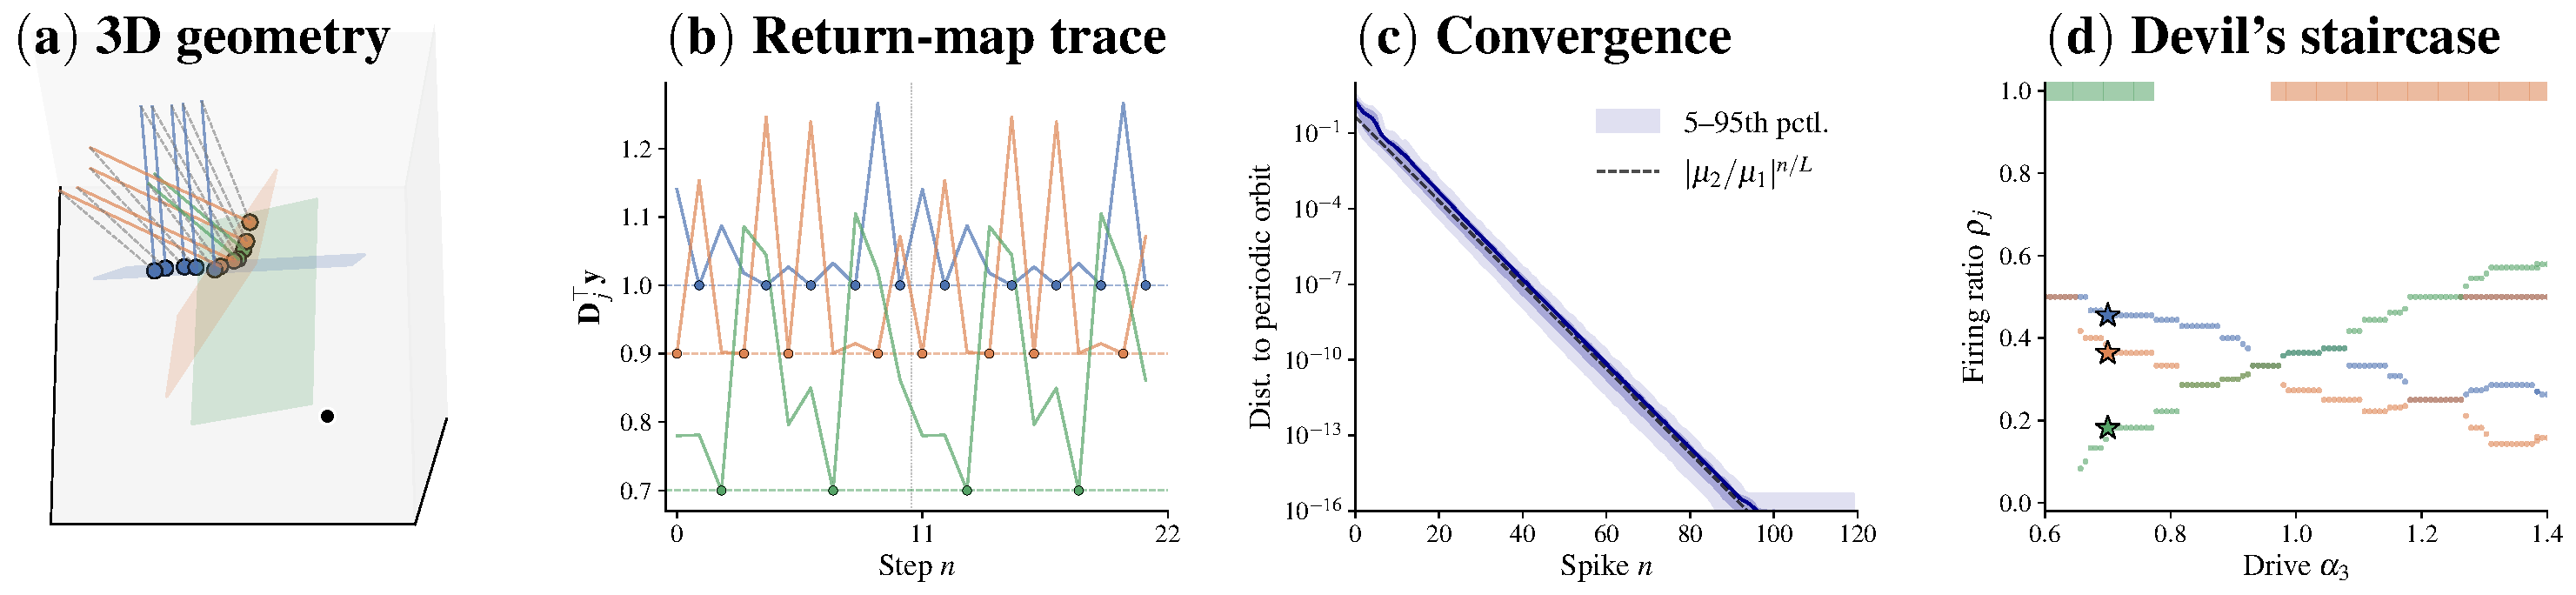
\includegraphics[width=\linewidth]{fig_3d_example_flat.pdf}
\end{minipage}\hfill
\begin{minipage}[t]{0.34\linewidth}\vspace{0pt}\raggedright
\colorbox{navy!7}{\parbox{\linewidth}{%
  \vspace{1mm}\normalsize
  \textbf{\color{navy}Aim:} Extend analysis to $N{\geq}2$. \textbf{\color{navy}Results:} The eigenvector prediction is exact at any $(K,N)$. Three features distinguish $K{\geq}3$ from $K{=}2$:
  
  \emph{1.~Stability:} $N{-}1$ eigenvalue ratios need to be checked rather than one.

  \emph{2.~Partition boundaries:} the borders between the self- and cross-return region on each bound are affine hyperplanes rather than points.

  \emph{3.~Multistability:} multi-bound cyclic orbit and self-trapping orbits coexist.
  
  \vspace{5mm}
  The $K{=}N{=}3$ example (\textbf{a}-\textbf{b}) verifies all $11$ orbit points to machine precision (\textbf{c}), with both stability ratios ($|\mu_2/\mu_1|=0.015$, $|\mu_3/\mu_1|=0.008$) are well inside the unit circle. Additionally, a scan over $\alpha_3$ (\textbf{d}) shows all firing ratios $\rho_j$ redistributing through mode-locked plateaus, confirming multisability.
  \vspace{1mm}
}}
\end{minipage}\hfill\mbox{}
\end{minipage}
}
\end{columns}


% ============================================================
% ROW 4: Chaos beyond the cone & Inverse Problem
% ============================================================
\begin{columns}
\column{0.55}
\block{\bt{5}{Order vs.\ Chaos}}{
\begin{minipage}[t]{\linewidth}
\centering
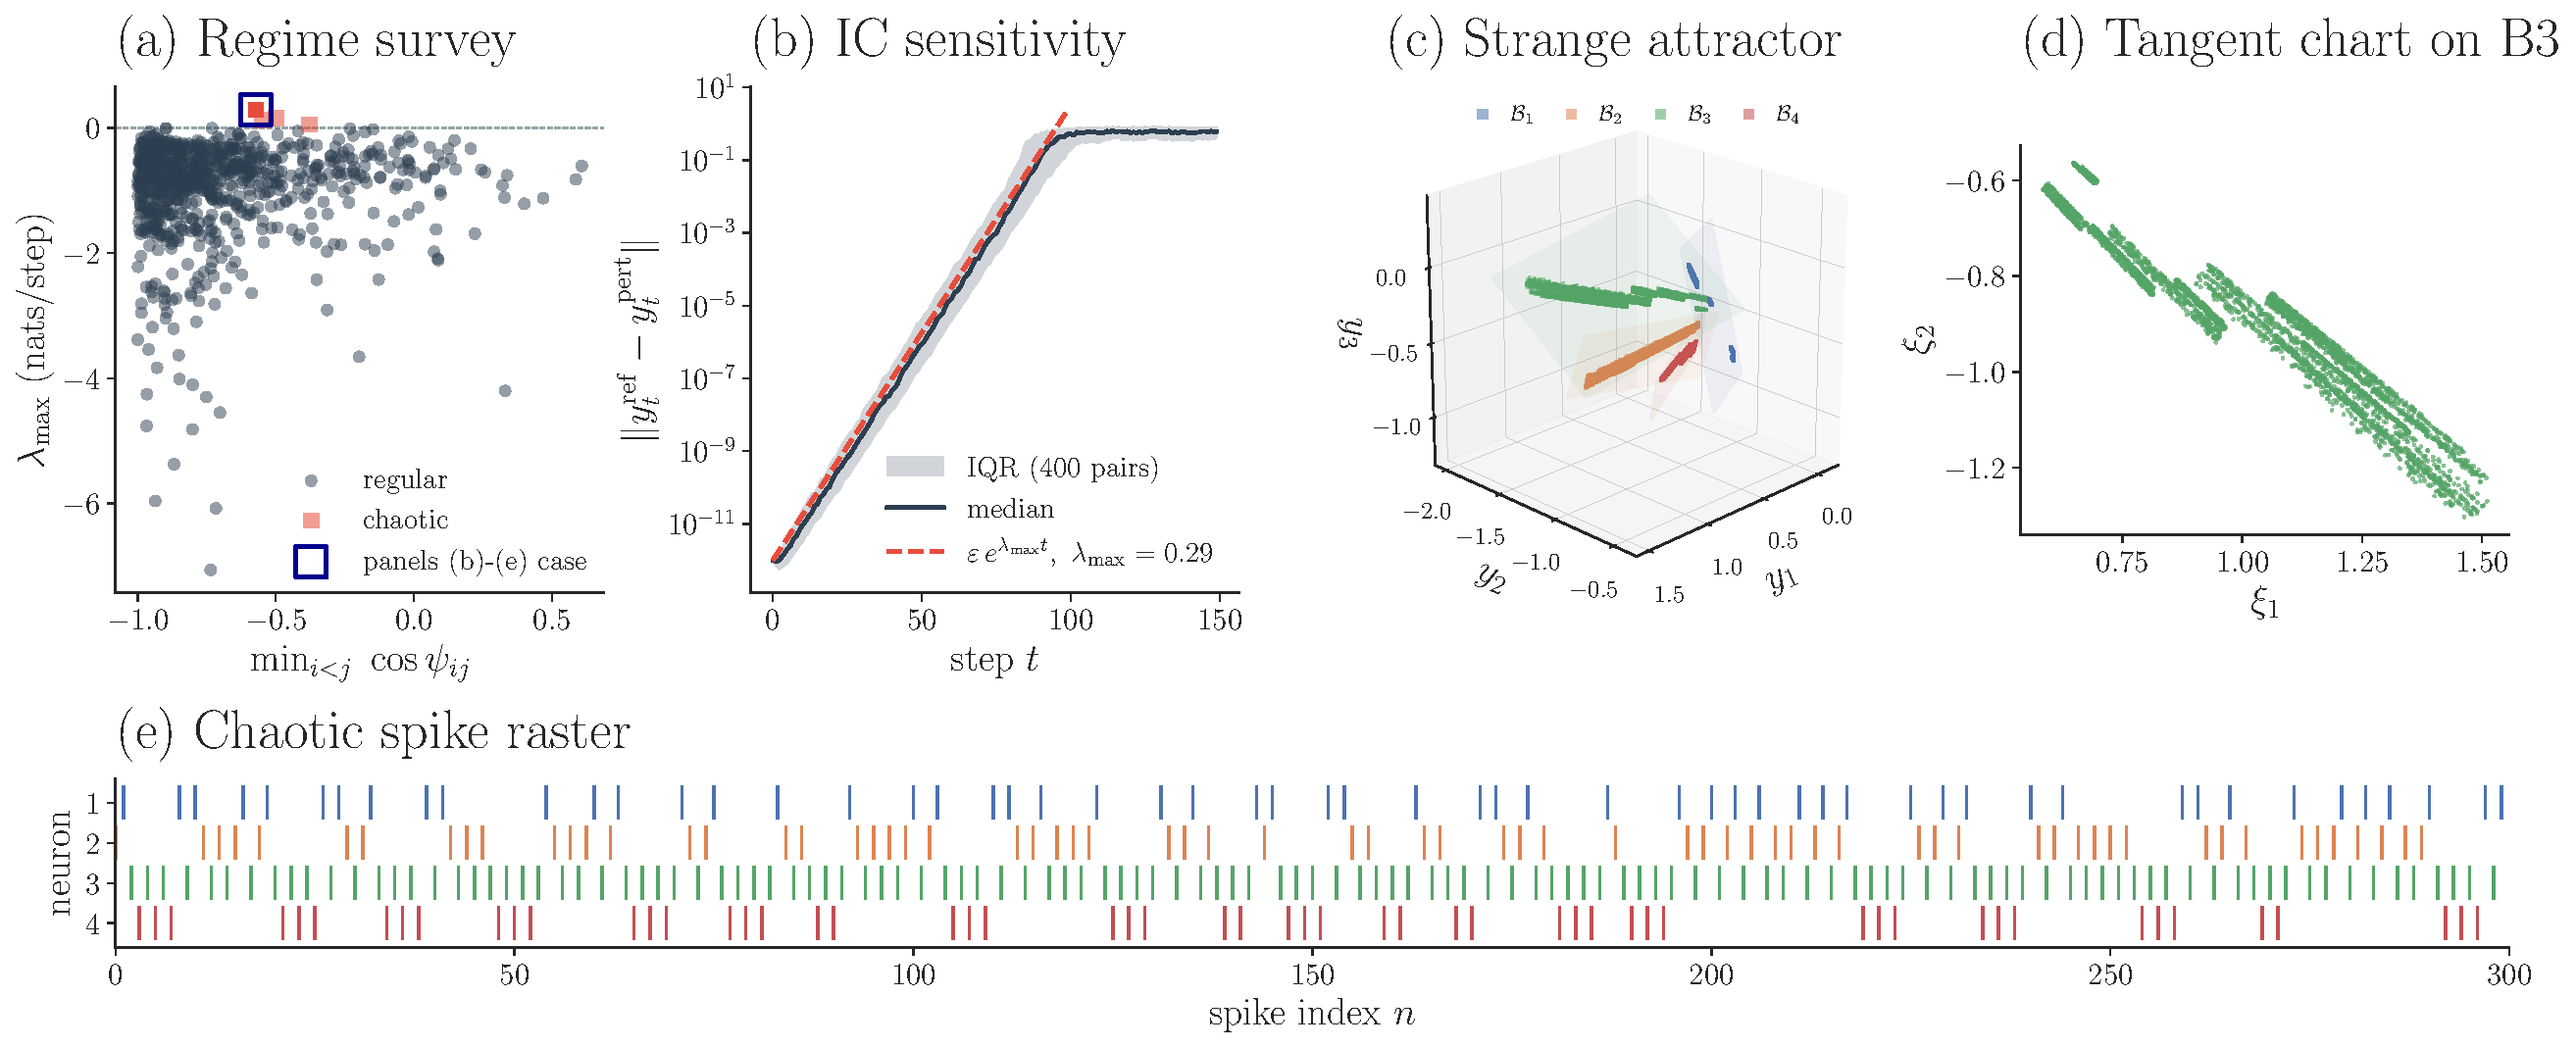
\includegraphics[width=0.91\linewidth]{chaos_figure.pdf}

\vspace{2mm}
\colorbox{navy!7}{\parbox{0.97\linewidth}{%
  \vspace{1mm}\normalsize
  \textbf{\color{navy}Aim:} Describe the conditions for chaotic behavior in SCNs.
  
  \vspace{1mm}
  \textbf{\color{navy}Results:}\;
  When all pairwise decoder cosines $\cos\psi_{ij}>0$ (uniformly inhibitory connectivity), the projective return map contracts the Hilbert metric on the positive cone: every admissible periodic orbit is stable, no chaos.
  A single negative cosine breaks the cone: an explicit $K{=}4$, $N{=}3$ SCN exhibits $\lambda_{\max}\approx 0.29$~nats/step with a strange attractor (panel~c).
  \emph{Biological analogue}: balanced inhibition-dominated cortex sits inside the stable cone; disinhibition pushes cosines negative, predicting the transition to irregular firing.
  \vspace{1.5mm}
}}
\end{minipage}
}

\column{0.45}
\block{\bt{6}{Inverse Problem}}{
\begin{minipage}[t]{\linewidth}\normalsize
\textbf{Aim:} Given an SCN find drives $\bm{\alpha}$ that realize a target spike sequence $\sigma$.

\vspace{1mm}
\textbf{Approach:} We define and maximize \textbf{admissibility margin} (competitor gap):
\begin{equation*}
m(\bm{\alpha}) = \min_{k}\;\bigl(
  c_{b_{k+1},k}(\bm{\alpha}) - \max_{j\neq b_{k+1}} c_{j,k(\bm{\alpha})}
\bigr),~\text{where}~c_{j,k}=\frac{\alpha_j}{\vv{D}^\top_j\vv{y}_k^+(\bm{\alpha})}~\text{(decay factor)}
\end{equation*}
  
\textbf{Results:} $m(\bm{\alpha})>0$ realizes the word; maximize $m(\bm{\alpha})$ for robustness.

\vspace{5mm}
% Two-panel row: admissibility landscape (aspect 2.170) + RBYGYB orbit
% (aspect 0.914 after fontsize=38 subtitle push made simon taller).
% Widths solve w_L / 2.170 = w_R / 0.914 with w_L + w_R = 0.96 →
% w_L = 0.676, w_R = 0.284, so BOTH panels render at the same on-poster
% height. minipage[t] anchors their tops together so the subtitle text
% (which sits at the top of each PDF after bbox_inches='tight') aligns.
\centering
\begin{minipage}[t]{0.9\linewidth}\raggedright
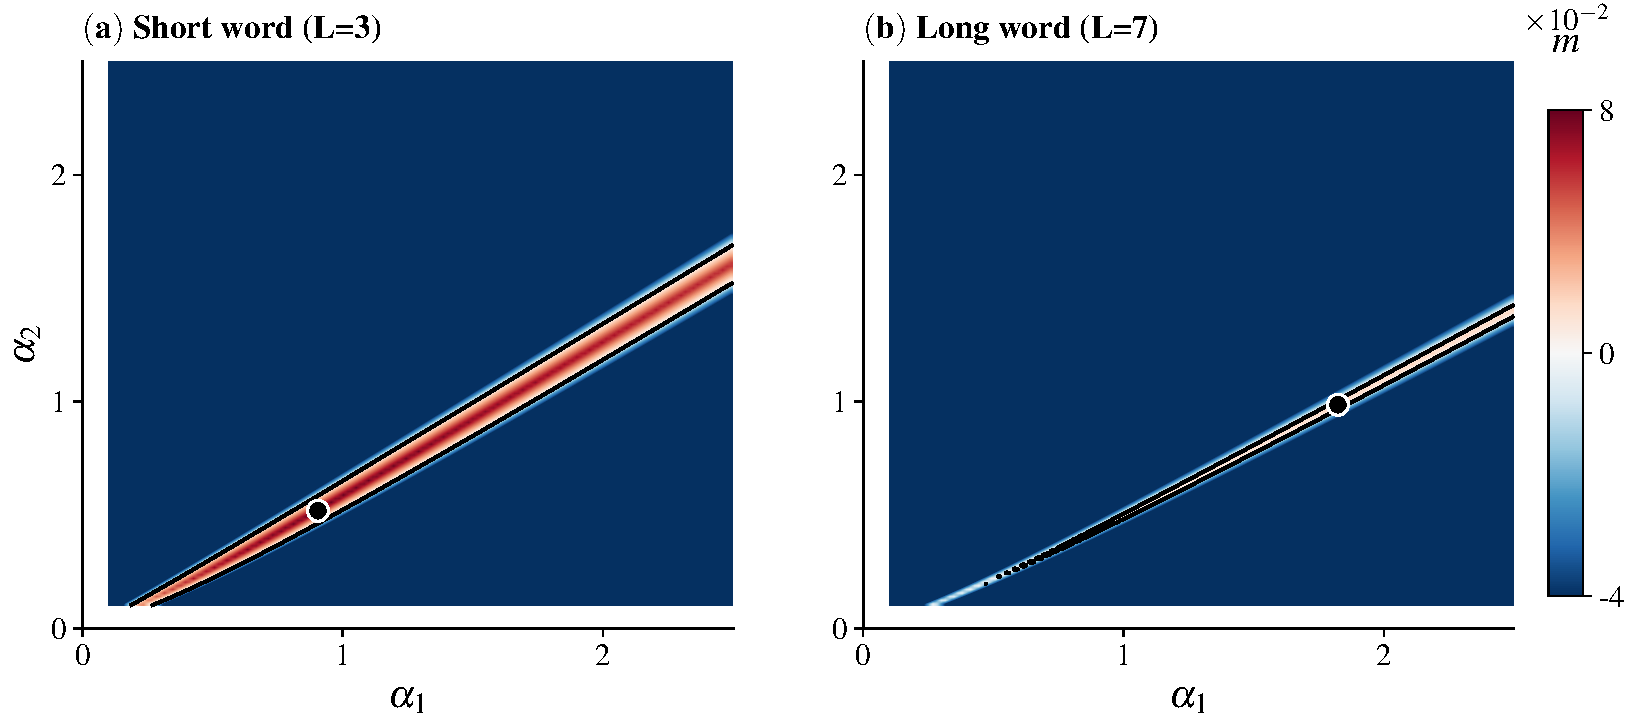
\includegraphics[width=0.676\linewidth]{margin_landscape.pdf}
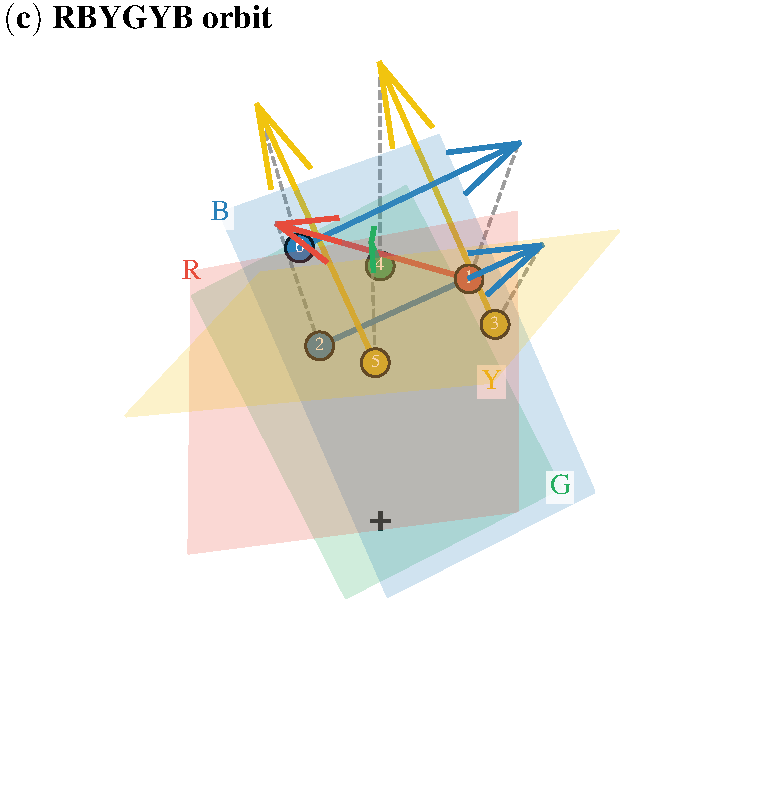
\includegraphics[width=0.284\linewidth]{simon_rbygyb.pdf}
\end{minipage}

\vspace{2mm}
{\centering
\setlength{\fboxsep}{2pt}%
\colorbox{navy!7}{\parbox{0.96\linewidth}{%
  \normalsize
  \textbf{\color{accent}Working memory:}\;
  Margin shrinks with sequence length which resembles the behavioral $4{\pm}1$ limit~\ref{ref:cowan}. \emph{Multistability}: varying the input $\xx$ navigates the staircase to switch between stored items.
  \emph{Storage is closed-form}: the drives $\bm{\alpha}$ are read off the linear program.
  \emph{Retrieval is autonomous}: each stored sequence is the leading eigenvector of the corresponding return map. %, so the orbit unfolds from any initial state in the basin.%
}}\par}

\vspace{2mm}
{\centering
\setlength{\fboxsep}{2pt}%
\colorbox{navy!7}{\parbox{0.96\linewidth}{%
  \vspace{1mm}\normalsize
  \textbf{\color{accent}Sequence memory (motor codes):}\;
  Precise motor sequences (e.g.\ songbird HVC syllable rasters~\ref{ref:hvc}) are naturally encoded as symbolic firing words $\sigma$: each syllable is one periodic word with its own return-map eigenvector. Syllable switches are drive-triggered basin transitions on a shared decoder $\vv{D}$. Storage cost scales with $KN$, not with sequence length: \textbf{one $K{=}10$, $N{=}50$ SCN carries $23$ coexisting stable words (periods $1$--$33$)}.%
  \vspace{1mm}
}}\par}
% No vspace: Box 6 with HVC callout is actually taller than Box 5 by
% ~1cm naturally; earlier "gap" measurements were confounded by Row 5's
% overlapping x-range. Leaving unpadded gives closest natural alignment.
\end{minipage}
}
\end{columns}

% ============================================================
% (Old Row 4: Sequence Memory) — merged into Box 6 above
% ROW 5: Bottom three blocks (pulled up slightly)
% ============================================================
% Pull the last row up (positive y = up). With Box 5/6 wrapped in 18cm
% fixed minipages there's now natural room; the previous 20mm pull-up
% cramped the last-row titles right against Row 4. Removing it lets
% tikzposter's default blockverticalspace (12mm) breathe.
% \makeatletter
% \global\advance\TP@blocktop by 20mm
% \global\TP@colbottom=\TP@blocktop
% \makeatother
\begin{columns}
\column{0.25}
\block{\btnonum{Takeaways}}{
\begin{minipage}[t][6cm][t]{\linewidth}\normalsize
\begin{itemize}[label={\color{accent}\textbullet}]
  \item Compile once ($O(K^2N^2)$), then query fast
  \item No simulation, no ODE solver
  \item Closed-form stability $|\mu_2/\mu_1|$
  \item Margin $m$ = closed-form robustness
  \item Inverse problem $\Rightarrow$ linear program for $\bm{\alpha}$
\end{itemize}
\end{minipage}
}
\column{0.25}
\block{\btnonum{Discussion}}{
\begin{minipage}[t][6cm][t]{\linewidth}\normalsize
\begin{itemize}[label={\color{accent}\textbullet}]
  \item Full-dim spike maps~\ref{ref:monteforte}; we add projective reduction
  \item Forced mode-locking~\ref{ref:coombes}; ours intrinsic
  \item UAP construction~ \ref{ref:podlaski},\ref{ref:sagodi26}
   \item No continuous attractors~\ref{ref:sagodi24}
  \item Chaos~\ref{ref:vreeswijk} if  $|\mu_2/\mu_1|\!>\!1$ % closed-form from the return-map spectrum
\end{itemize}
\end{minipage}
}
\column{0.5}
\block{\btnonum{References}}{
\begin{minipage}[t][6cm][t]{\linewidth}\small
\begin{multicols}{2}
\begin{enumerate}[label=\textbf{\color{accent}[\arabic*]}, leftmargin=*, itemsep=0pt, ref={[\arabic*]}]
  \item\label{ref:adrian} Adrian \& Zotterman, \emph{J. of Physiology} 1926
  \item \label{ref:hodgkin} Hodgkin \& Huxley, \emph{J. of Physiology} '52
  \item\label{ref:boerlin} Boerlin \emph{et al.}, \emph{PLoS CB} '13
  \item\label{ref:calaim} Calaim \emph{et al.}, \emph{eLife} '22
    \item\label{ref:arnold} Arnold, \emph{Izv.\ Akad.\ Nauk SSSR} '61
  \item\label{ref:herman} Herman, \emph{Publ.\ IH\'ES} '79
    \item\label{ref:cowan} Cowan, \emph{Behav.\ Brain Sci.} '01
  \item\label{ref:monteforte} Monteforte \& Wolf, \emph{PRX} '10
  \item\label{ref:coombes} Coombes \& Bressloff, \emph{PRE} '99
  \item\label{ref:podlaski} Podlaski \& Machens, \emph{Neural Comp.} '24
  \item\label{ref:sagodi26} S\'agodi \& Park, \emph{arXiv} '26
  \item \label{ref:sagodi24} S\'agodi \emph{et al.}, \emph{NeurIPS} '24
    \item\label{ref:vreeswijk} van Vreeswijk \& Sompolinsky, \emph{Sci.} '96
  \item\label{ref:hvc} Pascual \emph{et al.}, \emph{bioRxiv} '24
\end{enumerate}
\end{multicols}
\end{minipage}
}
\end{columns}

\begin{columns}
\column{1.0}
\block{}{
\centering
\includegraphics[width=0.8\linewidth]{FCT-Funding_Poster-A0-Footer_White_EN.png}
}
\end{columns}

\end{document}

% ==============================================================================
% COMPATIBILITY FIX (LaTeX 2024+ / TeX Live 2024–2026):
%
% ISSUE:
% Modern LaTeX kernels (since June 2024 / ltnews39) strictly forbid loading 
% packages or engine drivers inside a TeX group (\currentgrouplevel > 0). 
% Legacy `tikzposter` opens a group at \begin{document} via `\AtBeginDocument{\bgroup}`.
% Packages loaded in the preamble (like `mathtools` or `geometry`) defer setup code 
% or driver loading to \AtBeginDocument, which gets queued AFTER tikzposter's 
% \bgroup, causing them to load inside a group and trigger:
% "LaTeX Error: Loading a class or package in a group."
%
% SOLUTION:
% Pre-load affected packages BEFORE \documentclass using \RequirePackage{...}.
% This forces their \AtBeginDocument hooks to register BEFORE tikzposter 
% opens its group scope.
% ==============================================================================